\documentclass{ctexart}
\usepackage{ctex}
\usepackage{fontspec}
\usepackage[dvipsnames]{xcolor}
\usepackage{graphicx}
\usepackage{listings}
\lstset{
	language = Java,
	backgroundcolor = \color{DimGray!10},    % 背景色:淡黄
	basicstyle = \tiny\ttfamily,           % 基本样式 + 小号字体
	rulesepcolor= \color{gray},             % 代码块边框颜色
	breaklines = true,                  % 代码过长则换行
	numbers = left,                     % 行号在左侧显示
	numberstyle = \small,               % 行号字体
	keywordstyle = \color{blue},            % 关键字颜色
	commentstyle =\color{SpringGreen},        % 注释颜色
	stringstyle = \color{red!100},          % 字符串颜色
	frame = shadowbox,                  % 用(带影子效果)方框框住代码块
	showspaces = false,                 % 不显示空格
	columns = fixed,                    % 字间距固定
	%escapeinside={<@}{@>}              % 特殊自定分隔符:<@可以自己加颜色@>
	morekeywords = {as}               % 自加新的关键字(必须前后都是空格)      % 删除内定关键字;删除错误标记的关键字用deletekeywords删!
}
\title{\heiti \zihao{2} 简单的按钮计算器}
\date{\today}
\author{孙博言 \and 2011756 \and 计算机学院}
\begin{document}
\maketitle
本次作业采用了java swing图形化编程工具。下面我们首先介绍计算器的原理和功能。

Windows10内置计算器的标准模式,能够进行一般的日常运算,主要功能包括四则运算,乘方开根号等等。
\begin{itemize}
    \item 显示运算结果
    \item 以较高精度进行正确运算
    \item 归零退格等基本输入编辑功能
\end{itemize}
上述功能完成的核心,就是要设计好人机交互功能,主要是对按钮的事件响应函数进行编写,并且得到标准清晰的数字输出,向用户呈现。
现在,反复研究使用Winows计算器,熟悉它的逻辑功能,并且提炼出运行原理。我们不难得出以下特点.
\begin{itemize}
    \item 计算器内部只存储运算结果和输入结果两个数据域。
    \item 按键数字输入永远针对输入结果数据进行后缀式添加。
    \item 运算符分为根据逻辑功能分为以下三类:
          \begin{itemize}
              \item 单目运算符:$\%$,$x^2$,$\sqrt{x}$,$\pm$
              \item 双目运算符:$+$,$-$,$\times$,$\div$
              \item 特殊的等号运算符:$=$
          \end{itemize}
    \item 异常输入运算结果简单式处理。
    \item 全部清零C和表达式清零CE。
\end{itemize}
\newpage
\begin{figure}[htbp]
    \centering
    \caption{Windows10计算器截图}
    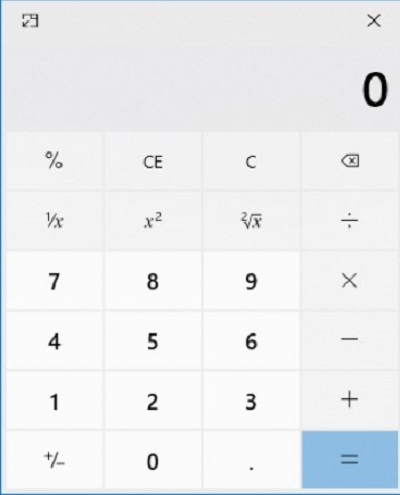
\includegraphics{1.jpg}
    \label{fig:1}
\end{figure}
我们新建一个calculator类,绘制Frame,button等代码在此不再赘述,重点分析运算逻辑。
\begin{itemize}
    \item \textcolor{blue}{\fontspec{Consolas} BigDecimal}类型的\textcolor{blue}{\fontspec{Consolas} result}对象。
    \item \textcolor{blue}{\fontspec{Consolas} BigDecimal}类型的\textcolor{blue}{\fontspec{Consolas} inNum}对象。
\end{itemize}
分别用来存储计算器中的结果和输入数据。\textcolor{blue}{\fontspec{Consolas} inNum}通过\textcolor{blue}{\fontspec{Consolas} StringBuilder}类型的对象为参数进行构造。
按下数字按钮时后缀相应的数字。

接下来进行关键的分析:操作焦点切换。

一般情况下,当按下双目运算符时系统的处理动作相同,首先系统要计算上一个运算符对应的运算,操作数为\textcolor{blue}{\fontspec{Consolas} inNum}和\textcolor{blue}{\fontspec{Consolas} result},并且把运算结果存入\textcolor{blue}{\fontspec{Consolas} result}。\textcolor{blue}{\fontspec{Consolas} inNum}不变,操作符更新为新按下的运算符。

但是当按下等号之后情况发生了变化。按下等号后执行上一步的运算,不更新运算符,\textcolor{blue}{\fontspec{Consolas} result}更新,\textcolor{blue}{\fontspec{Consolas} inNum}的实际数值暂时不变,输入区清零,标签显示结果。
之后视用户首次操作产生不同的响应:
\begin{itemize}
    \item 若用户首先按下的是数字,则整个输入的数字字符串存入\textcolor{blue}{\fontspec{Consolas} result}当中,\textcolor{blue}{\fontspec{Consolas} inNum}和运算符不变。
    \item 若用户首先按下的是双目运算符,则\textcolor{blue}{\fontspec{Consolas} result}赋值给\textcolor{blue}{\fontspec{Consolas} inNum},运算符更新为新按下的运算符。
    \item 若用户按下的是等号,则执行上一步的运算,运算结果存入\textcolor{blue}{\fontspec{Consolas} result},\textcolor{blue}{\fontspec{Consolas} inNum}不变,重新返回。
\end{itemize}
这些逻辑在设计初期就被发现,并且完整复现到了程序当中。

下面,要考虑到功能十分特殊的单目运算符的情况,它们的逻辑比较不同寻常,并不会像双目运算符一样按下后暂时存储。
\begin{itemize}
    \item 若上一步按下的是等号则:作用于运算结果\textcolor{blue}{\fontspec{Consolas} result},当前焦点变为\textcolor{blue}{\fontspec{Consolas} result}。\textcolor{blue}{\fontspec{Consolas} inNum}和上一步运算符不变。
    \item 若上一步按下的是数字则:作用\textcolor{blue}{\fontspec{Consolas} inNum},不影响\textcolor{blue}{\fontspec{Consolas} result},并且进入到类似于按下等号之后的失去输入焦点状态,输入字符串被清零。
    \item 若上一步按下的是除了等号外的其他双目运算符:运算作用于\textcolor{blue}{\fontspec{Consolas} result},但是实际上赋值给\textcolor{blue}{\fontspec{Consolas} inNum}。
    \item 若上一步按下的是单目运算符:则作用于所谓的上一步操作影响到的数据域!改变它的值!
\end{itemize}
{\heiti \zihao{4} 另外事实上,{\%}这一运算符不完全类似于以上任何一种……}

上一步完成的是的是乘除法运算的话,运算就实际上是除以100。但如果是加减法运算,就要将第一个加数加上两个加数相乘在除以100。
类似于小费的计算。可能是一种经济学中的习惯。在此之中不可避免地需要用到第三个数据域,因为在进行下列表达式时你会注意到这个必要性。

这些逻辑为个人一步步尝试不同的按键组合得出,其实质是操作焦点的问题,对当下数据域产生何种影响,依据的是那一块数据域,并且对另一块数据域产生不同影响。

比如以下比较特殊的操作,可供比照参考:

$x+y+===$;$x\times y===$;$x+y=z=$;$x+y=+==$;
$x+y\pm\pm=$;$x+y\%=$;$x+y=\%$;$x+y=\%\%$;$x+y=$ $\sqrt{\quad}$ $\%$;
$x+y=\%+=$;$x+y=\%==$;


{\heiti \zihao{3} 其余操作不再赘述,但是有一些细节}

\begin{itemize}
    \item 除以零或者出现复数显示为非法。
    \item 表达式清零与全部清零代表不同含义。
    \item 退格对输入串操作为退格,对结果串操作为清零。
    \item 结果不是小数不会显示多余的零。
    \item 但是实验中出现过一些精度无法正确显示的问题,因为字符串不能过长。
    \item ……
\end{itemize}

以下为所有的代码和运行截图:

\begin{figure}[htbp]
    \centering
    \caption{负数开根号}\label{fig:2}
    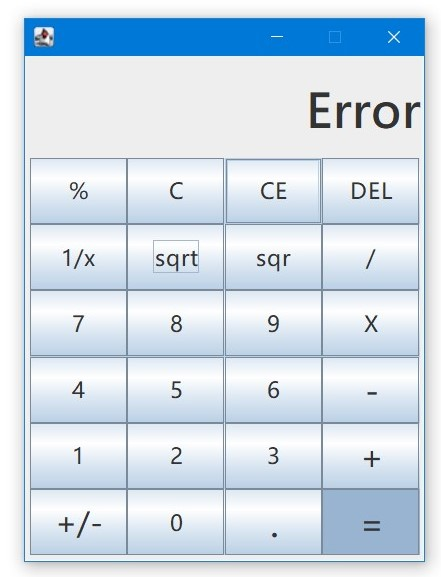
\includegraphics[scale=0.7]{3.jpg}
\end{figure}
\newpage
\begin{figure}[htbp]
    \centering
    \caption{除以零}\label{fig:3}
    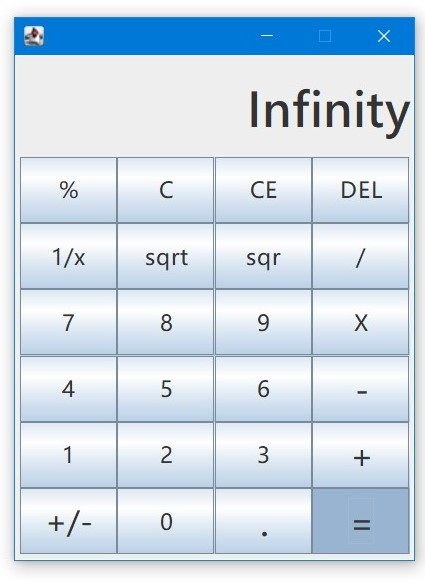
\includegraphics[scale=0.50]{4.jpg} 
\end{figure}
\begin{figure}[htbp]
    \centering
    \caption{$8+9=\sqrt{\quad}\%$的运算结果}\label{fig:4}
    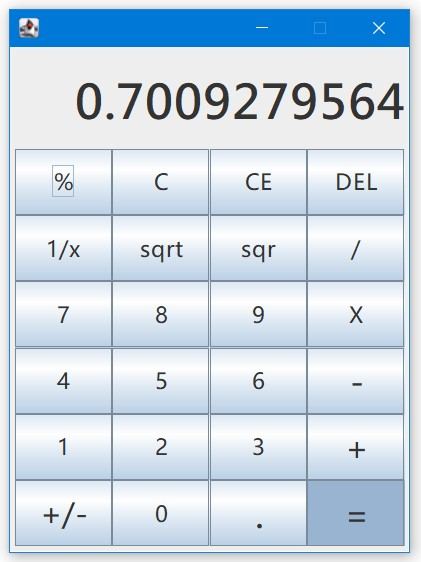
\includegraphics[scale=0.50]{5.jpg} 
\end{figure}
这可能一开始会令人吃惊……
\begin{figure}[htbp]
    \centering
    \caption{$8+9=\sqrt{\quad}\%$win10的运算结果}\label{fig:4}
    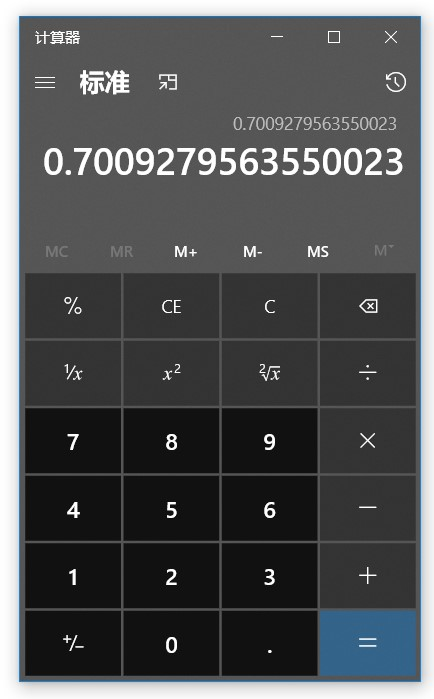
\includegraphics[scale=1.2]{6.jpg} 
\end{figure}
\newpage
可直接复制粘贴运行,把package名字改掉。
{\kaishu \zihao{3} 源码放在}
\begin{lstlisting}[caption=冗杂的代码]
    package sunboyan;

    import java.awt.BorderLayout;
    import java.awt.EventQueue;
    import javax.swing.JFrame;
    import javax.swing.JPanel;
    import javax.swing.border.EmptyBorder;
    import javax.swing.JLabel;
    import java.awt.Font;
    import java.awt.GridLayout;
    import javax.swing.JButton;
    import javax.swing.SwingConstants;
    import java.awt.event.MouseAdapter;
    import java.awt.event.MouseEvent;
    import java.math.*;
    import java.awt.SystemColor;
    import javax.swing.UIManager;
    public class Calculator extends JFrame {
        
        private static final long serialVersionUID = 1L;
        BigDecimal result=new BigDecimal(0);
        String resultString=new String("0");
        BigDecimal inNum=new BigDecimal(0);
        StringBuilder inString=new StringBuilder("0");
        BigDecimal perTemp=new BigDecimal(0);
        char operatorString=' ';
        boolean equaled=false;
        boolean dotted=false;	
        boolean computed=false;
        private JPanel contentPane;
        public JLabel myResultLabel;
        public static void main(String[] args) {
            EventQueue.invokeLater(new Runnable() {
                public void run() {
                    try {
                        Calculator frame = new Calculator();
                        frame.setVisible(true);
                    } catch (Exception e) {
                        e.printStackTrace();
                    }
                }
            });
        }
        public Calculator() {
            setResizable(false);
            setDefaultCloseOperation(JFrame.EXIT_ON_CLOSE);
            setBounds(0, 0, 334, 442);
            contentPane = new JPanel();
            contentPane.setBackground(SystemColor.control);
            contentPane.setBorder(new EmptyBorder(2, 3, 2, 3));
            contentPane.setLayout(new BorderLayout(0, 0));
            setContentPane(contentPane);
            
            JPanel downPanel = new JPanel();
            downPanel.setBorder(new EmptyBorder(0, 0, 0, 0));
            contentPane.add(downPanel, BorderLayout.CENTER);
            downPanel.setLayout(new GridLayout(6, 4, 0, 0));
            
            JButton percentButton = new JButton("%");
            percentButton.setFont(new Font("微软雅黑", Font.PLAIN, 18));
            percentButton.addMouseListener(new MouseAdapter() {
                @Override
                public void mouseReleased(MouseEvent e) {
                    if(equaled) {
                        System.out.println(perTemp);
                        System.out.println(inNum);
                        System.out.println(result);
                            if (computed) {
                                if (operatorString == '+' || operatorString == '-') {
                                    perTemp=result;
                                    result=result.multiply(perTemp).divide(new BigDecimal("100.0"),10,RoundingMode.HALF_UP);
                                    computed=false;
                                } else {
                                    result = result.divide(new BigDecimal("100.0"), 10, RoundingMode.HALF_UP);
                                }
                                result.setScale(10, RoundingMode.HALF_UP);
                                if (result.compareTo(new BigDecimal(result.intValue())) == 0) {
                                    resultString = String.valueOf(result.intValue());
                                } else {
                                    resultString = result.stripTrailingZeros().toString();
                                }
                                inString.delete(0, inString.length());
                                if (resultString.length() < 14) {
                                    myResultLabel.setText(resultString.toString());
                                } else {
                                    myResultLabel.setText(resultString.toString().substring(0, 14));
                                } 
                            } else {
                                if (operatorString == '+' || operatorString == '-') {
                                    result=result.multiply(perTemp).divide(new BigDecimal("100.0"),10,RoundingMode.HALF_UP);
                                } else {
                                    result = result.divide(new BigDecimal("100.0"), 10, RoundingMode.HALF_UP);
                                }
                                result.setScale(10, RoundingMode.HALF_UP);
                                if (result.compareTo(new BigDecimal(result.intValue())) == 0) {
                                    resultString = String.valueOf(result.intValue());
                                } else {
                                    resultString = result.stripTrailingZeros().toString();
                                }
                                inString.delete(0, inString.length());
                                if (resultString.length() < 14) {
                                    myResultLabel.setText(resultString.toString());
                                } else {
                                    myResultLabel.setText(resultString.toString().substring(0, 14));
                                } 
                            }
                    }else {
                        if (computed) {
                            if (operatorString=='+'||operatorString=='-') {
                                System.out.println(4);
                                result = perTemp.multiply(result).divide(new BigDecimal("100.0"), 10, RoundingMode.HALF_UP);
                            }else {
                                inNum = result.divide(new BigDecimal("100.0"), 10, RoundingMode.HALF_UP);
                            }
                            result.setScale(10, RoundingMode.HALF_UP);
                            if (result.compareTo(new BigDecimal(result.intValue())) == 0) {
                                resultString = String.valueOf(result.intValue());
                            } else {
                                resultString = result.stripTrailingZeros().toString();
                            }
                            inString.delete(0, inString.length());
                            if (resultString.length() < 14) {
                                myResultLabel.setText(resultString.toString());
                            } else {
                                myResultLabel.setText(resultString.toString().substring(0, 14));
                            } 
                        }else {
                            if (operatorString=='+'||operatorString=='-') {
                                System.out.println(5);
                                inNum = inNum.multiply(result).divide(new BigDecimal("100.0"), 10,
                                        RoundingMode.HALF_UP);
                            }else {
                                inNum = inNum.divide(new BigDecimal("100.0"), 10,
                                        RoundingMode.HALF_UP);
                            }
                            result.setScale(10, RoundingMode.HALF_UP);
                            if (inNum.compareTo(new BigDecimal(inNum.intValue())) == 0) {
                                resultString = String.valueOf(inNum.intValue());
                            } else {
                                resultString = inNum.stripTrailingZeros().toString();
                            }
                            inString.delete(0, inString.length());
                            if (resultString.length() < 14) {
                                myResultLabel.setText(resultString.toString());
                            } else {
                                myResultLabel.setText(resultString.toString().substring(0, 14));
                            }
                        }
                    }
                    computed=false;
                }
            });
            downPanel.add(percentButton);
            
            JButton clearButton = new JButton("C");
            clearButton.setFont(new Font("微软雅黑", Font.PLAIN, 18));
            clearButton.addMouseListener(new MouseAdapter() {
                @Override
                public void mouseReleased(MouseEvent e) {
                    perTemp=new BigDecimal("0");
                    equaled=false;
                    inNum=new BigDecimal("0");
                    result=new BigDecimal("0");
                    inString.replace(0,inString.length(),"0");
                    resultString="0";
                    dotted=false;
                    operatorString=' ';
                    myResultLabel.setText("0");
                }
            });
            downPanel.add(clearButton);
            
            JButton cClearButton = new JButton("CE");
            cClearButton.setFont(new Font("微软雅黑", Font.PLAIN, 18));
            cClearButton.addMouseListener(new MouseAdapter() {
                @Override
                public void mouseReleased(MouseEvent e) {
                    perTemp=new BigDecimal("0");
                    if(equaled) {
                        inString.delete(0, inString.length());
                        myResultLabel.setText("0");
                        result = new BigDecimal("0");
                        dotted=false;
                    }else {
                        inString.delete(0, inString.length());
                        myResultLabel.setText("0");
                        inNum=new BigDecimal("0");
                        dotted=false;
                    }		
                }
            });
            downPanel.add(cClearButton);
            
            JButton backButton = new JButton("DEL");
            backButton.setFont(new Font("微软雅黑", Font.PLAIN, 18));
            backButton.addMouseListener(new MouseAdapter() {
                @Override
                public void mouseReleased(MouseEvent e) {
                    if(equaled) {
                        ;
                    }else {
                        if(inString.length()>1) {
                            if(inString.charAt(inString.length()-1)=='.')
                            {
                                inString.delete(inString.length()-1, inString.length());
                            }
                            inString.delete(inString.length()-1, inString.length());
                            inNum=new BigDecimal(inString.toString());
                            if(inNum.compareTo(new BigDecimal(inNum.intValue()))==0){
                                resultString=String.valueOf(inNum.intValue());
                            }else {
                                resultString = inNum.stripTrailingZeros().toString();
                            }
                            if (resultString.length()<14) {
                                myResultLabel.setText(resultString.toString());
                            }else {
                                myResultLabel.setText(resultString.toString().substring(0,14));
                            }
                        }else {
                            inString.replace(0, 1, "0");
                            inNum=new BigDecimal(inString.toString());
                            if(inNum.compareTo(new BigDecimal(inNum.intValue()))==0){
                                resultString=String.valueOf(inNum.intValue());
                            }else {
                                resultString = inNum.stripTrailingZeros().toString();
                            }
                            if (resultString.length()<14) {
                                myResultLabel.setText(resultString.toString());
                            }else {
                                myResultLabel.setText(resultString.toString().substring(0,14));
                            }
                        }
                    }
                }
            });
            downPanel.add(backButton);
            
            JButton dButton = new JButton("1/x");
            dButton.setFont(new Font("微软雅黑", Font.PLAIN, 18));
            dButton.addMouseListener(new MouseAdapter() {
                @Override
                public void mouseReleased(MouseEvent e) {
                    if(equaled) {
                        if(result.equals(new BigDecimal("0"))) {
                            resultString="Infinity";
                            //pause
                        }else {
                            perTemp=new BigDecimal(result.toString());
                            result = new BigDecimal("1").divide(result,10, RoundingMode.HALF_DOWN);
                            result.setScale(10,RoundingMode.HALF_UP);
                            if(result.compareTo(new BigDecimal(result.intValue()))==0){
                                resultString=String.valueOf(result.intValue());
                            }else {
                                resultString = result.stripTrailingZeros().toString();
                            }
                        }
                        computed=true;
                        inString.delete(0, inString.length());
                        if (resultString.length()<14) {
                            myResultLabel.setText(resultString.toString());
                        }else {
                            myResultLabel.setText(resultString.toString().substring(0,14));
                        }
                    }else {
                        if (computed) {
                            if (inNum.equals(new BigDecimal("0"))) {
                                resultString = "Infinity";
                                //pause
                            } else {
                                perTemp=new BigDecimal(result.toString());
                                inNum = new BigDecimal("1").divide(result, 10, RoundingMode.HALF_DOWN);
                                inNum.setScale(10, RoundingMode.HALF_UP);
                                if (inNum.compareTo(new BigDecimal(inNum.intValue())) == 0) {
                                    resultString = String.valueOf(inNum.intValue());
                                } else {
                                    resultString = inNum.stripTrailingZeros().toString();
                                }
                            }
                            inString.delete(0, inString.length());
                            if (resultString.length() < 14) {
                                myResultLabel.setText(resultString.toString());
                            } else {
                                myResultLabel.setText(resultString.toString().substring(0, 14));
                            } 
                        }else {
                            if (inNum.equals(new BigDecimal("0"))) {
                                resultString = "Infinity";
                                backButton.setEnabled(false);
                            } else {
                                perTemp=new BigDecimal(inNum.toString());
                                inNum = new BigDecimal("1").divide(inNum, 10, RoundingMode.HALF_DOWN);
                                inNum.setScale(10, RoundingMode.HALF_UP);
                                if (inNum.compareTo(new BigDecimal(inNum.intValue())) == 0) {
                                    resultString = String.valueOf(inNum.intValue());
                                } else {
                                    resultString = inNum.stripTrailingZeros().toString();
                                }
                            }
                            inString.delete(0, inString.length());
                            if (resultString.length() < 14) {
                                myResultLabel.setText(resultString.toString());
                            } else {
                                myResultLabel.setText(resultString.toString().substring(0, 14));
                            } 
                        }
                    }
                computed=false;	
                }
            });
            downPanel.add(dButton);		
            JButton squareButton = new JButton("sqrt");
            squareButton.setFont(new Font("微软雅黑", Font.PLAIN, 18));
            squareButton.addMouseListener(new MouseAdapter() {
                @Override
                public void mouseReleased(MouseEvent e) {
                    if(equaled) {
                        try {
                            perTemp=new BigDecimal(result.toString());
                            result = result.sqrt(MathContext.DECIMAL64);
                        } catch (Exception e2) {
                            myResultLabel.setText("Error");
                            return;
                        }
                        result.setScale(10, RoundingMode.HALF_UP);
                        if(result.compareTo(new BigDecimal(result.intValue()))==0){
                            resultString=String.valueOf(result.intValue());
                        }else {
                            resultString = result.stripTrailingZeros().toString();
                        }
                        inString.delete(0, inString.length());
                        if (resultString.length()<14) {
                            myResultLabel.setText(resultString.toString());
                        }else {
                            myResultLabel.setText(resultString.toString().substring(0,14));
                        }
                    }else {
                        if (computed) {
                            try {
                                perTemp=new BigDecimal(result.toString());
                                inNum = result.sqrt(MathContext.DECIMAL64);
                            } catch (Exception e2) {
                                myResultLabel.setText("Error");
                                return;
                            }
                            result.setScale(10, RoundingMode.HALF_UP);
                            if (inNum.compareTo(new BigDecimal(result.intValue())) == 0) {
                                resultString = String.valueOf(inNum.intValue());
                            } else {
                                resultString = inNum.stripTrailingZeros().toString();
                            }
                            inString.delete(0, inString.length());
                            if (resultString.length() < 14) {
                                myResultLabel.setText(resultString.toString());
                            } else {
                                myResultLabel.setText(resultString.toString().substring(0, 14));
                            } 
                        }else {
                            try {
                                perTemp=new BigDecimal(inNum.toString());
                                inNum = inNum.sqrt(MathContext.DECIMAL64);
                            } catch (Exception e2) {
                                myResultLabel.setText("Error");
                                return;
                            }
                            result.setScale(10, RoundingMode.HALF_UP);
                            if (inNum.compareTo(new BigDecimal(inNum.intValue())) == 0) {
                                resultString = String.valueOf(inNum.intValue());
                            } else {
                                resultString = inNum.stripTrailingZeros().toString();
                            }
                            inString.delete(0, inString.length());
                            if (resultString.length() < 14) {
                                myResultLabel.setText(resultString.toString());
                            } else {
                                myResultLabel.setText(resultString.toString().substring(0, 14));
                            } 
                        }
                    }
                    computed=false;	
                }
                
            });
            downPanel.add(squareButton);
            
            JButton sqrtButton = new JButton("sqr");
            sqrtButton.setFont(new Font("微软雅黑", Font.PLAIN, 18));
            sqrtButton.addMouseListener(new MouseAdapter() {
                @Override
                public void mouseReleased(MouseEvent e) {
                    if(equaled) {
                        perTemp=new BigDecimal(result.toString());
                        result=result.pow(2);
                        result.setScale(10, RoundingMode.HALF_UP);
                        if(result.compareTo(new BigDecimal(result.intValue()))==0){
                            resultString=String.valueOf(result.intValue());
                        }else {
                            resultString = result.stripTrailingZeros().toString();
                        }
                        inString.delete(0, inString.length());
                        if (resultString.length()<14) {
                            myResultLabel.setText(resultString.toString());
                        }else {
                            myResultLabel.setText(resultString.toString().substring(0,14));
                        }
                    }else {
                        if (computed) {
                            perTemp=new BigDecimal(result.toString());
                            inNum = result.pow(2);
                            result.setScale(10, RoundingMode.HALF_UP);
                            if (inNum.compareTo(new BigDecimal(inNum.intValue())) == 0) {
                                resultString = String.valueOf(inNum.intValue());
                            } else {
                                resultString = inNum.stripTrailingZeros().toString();
                            }
                            inString.delete(0, inString.length());
                            if (resultString.length() < 14) {
                                myResultLabel.setText(resultString.toString());
                            } else {
                                myResultLabel.setText(resultString.toString().substring(0, 14));
                            } 
                        }else {
                            perTemp=new BigDecimal(inNum.toString());
                            inNum = inNum.pow(2);
                            result.setScale(10, RoundingMode.HALF_UP);
                            if (inNum.compareTo(new BigDecimal(inNum.intValue())) == 0) {
                                resultString = String.valueOf(inNum.intValue());
                            } else {
                                resultString = inNum.stripTrailingZeros().toString();
                            }
                            inString.delete(0, inString.length());
                            if (resultString.length() < 14) {
                                myResultLabel.setText(resultString.toString());
                            } else {
                                myResultLabel.setText(resultString.toString().substring(0, 14));
                            }
                        }
                    }	
                    computed=false;	
                }
            });
            downPanel.add(sqrtButton);
            
            JButton divideButton = new JButton("/");
            divideButton.setFont(new Font("微软雅黑", Font.PLAIN, 18));
            divideButton.addMouseListener(new MouseAdapter() {
                @Override
                public void mouseReleased(MouseEvent e) {
                    perTemp=new BigDecimal("0");
                    if(equaled) {
                        inNum = new BigDecimal(result.toString());
                        inString.delete(0, inString.length());
                        operatorString='/';
                        equaled=false;
                        if (resultString.length()<14) {
                            myResultLabel.setText(resultString.toString());
                        }else {
                            myResultLabel.setText(resultString.toString().substring(0,14));
                        }
                    }else {
                        compute();
                        inString.delete(0, inString.length());
                        operatorString='/';
                        if (resultString.length()<14) {
                            myResultLabel.setText(resultString.toString());
                        }else {
                            myResultLabel.setText(resultString.toString().substring(0,14));
                        }
                    }		
                }
            });
            downPanel.add(divideButton);
            
            JButton sevenButton = new JButton("7");
            sevenButton.setFont(new Font("微软雅黑", Font.PLAIN, 18));
            sevenButton.addMouseListener(new MouseAdapter() {
                @Override
                public void mouseReleased(MouseEvent e) {
                    perTemp=new BigDecimal("0");
                    computed=false;
                    if(inString.length()==1&&inString.charAt(0)=='0') {
                        inString.delete(0, 1);
                    }
                    inString.append('7');
                    if (equaled) {
                        result = new BigDecimal(inString.toString());		
                    } else {
                        inNum=new BigDecimal(inString.toString());
                    }
                    if (inString.length() < 14) {
                            myResultLabel.setText(inString.toString());
                    } 
                }
            
            });
            downPanel.add(sevenButton);
            
            JButton eightButton = new JButton("8");
            eightButton.addMouseListener(new MouseAdapter() {
                @Override
                public void mouseReleased(MouseEvent e) {
                    perTemp=new BigDecimal("0");
                    computed=false;
                    if(inString.length()==1&&inString.charAt(0)=='0') {
                        inString.delete(0, 1);
                    }
                    inString.append('8');
                    if (equaled) {
                        result = new BigDecimal(inString.toString());		
                    } else {
                        inNum=new BigDecimal(inString.toString());
                    }
                    if (inString.length()<14) {
                        myResultLabel.setText(inString.toString());
                    }
                }
            
            });
            downPanel.add(eightButton);
            eightButton.setFont(new Font("微软雅黑", Font.PLAIN, 18));
            
            JButton nineButton = new JButton("9");
            nineButton.addMouseListener(new MouseAdapter() {
                @Override
                public void mouseReleased(MouseEvent e) {
                    perTemp=new BigDecimal("0");
                    computed=false;
                    if(inString.length()==1&&inString.charAt(0)=='0') {
                        inString.delete(0, 1);
                    }
                    inString.append('9');
                    if (equaled) {
                        result = new BigDecimal(inString.toString());		
                    } else {
                        inNum=new BigDecimal(inString.toString());
                    }
                    if (inString.length()<14) {
                        myResultLabel.setText(inString.toString());
                    }			
                }
            
            });
            nineButton.setFont(new Font("微软雅黑", Font.PLAIN, 18));
            downPanel.add(nineButton);
            
            JButton multiButton = new JButton("X");
            multiButton.addMouseListener(new MouseAdapter() {
                @Override
                public void mouseReleased(MouseEvent e) {
                    perTemp=new BigDecimal("0");
                    if(equaled) {
                        inNum = new BigDecimal(result.toString());
                        System.out.println("11");
                        inString.delete(0, inString.length());
                        operatorString='*';
                        equaled=false;
                        if (resultString.length()<14) {
                            myResultLabel.setText(resultString.toString());
                        }else {
                            myResultLabel.setText(resultString.toString().substring(0,14));
                        }
                    }else {
                        compute();
                        inString.delete(0, inString.length());
                        operatorString='*';
                        if (resultString.length()<14) {
                            myResultLabel.setText(resultString.toString());
                        }else {
                            myResultLabel.setText(resultString.toString().substring(0,14));
                        }
                    }
                }
            });
            multiButton.setFont(new Font("微软雅黑", Font.PLAIN, 18));
            downPanel.add(multiButton);
            
            JButton fourButton = new JButton("4");
            fourButton.addMouseListener(new MouseAdapter() {
                @Override
                public void mouseReleased(MouseEvent e) {
                    perTemp=new BigDecimal("0");
                    computed=false;
                    if(inString.length()==1&&inString.charAt(0)=='0') {
                        inString.delete(0, 1);
                    }
                    inString.append('4');
                    if (equaled) {
                        result = new BigDecimal(inString.toString());		
                    } else {
                        inNum=new BigDecimal(inString.toString());
                    }
                    if (inString.length()<14) {
                        myResultLabel.setText(inString.toString());
                    }
                }
            
            });
            fourButton.setFont(new Font("微软雅黑", Font.PLAIN, 18));
            downPanel.add(fourButton);
            
            JButton fiveButton = new JButton("5");
            fiveButton.addMouseListener(new MouseAdapter() {
                @Override
                public void mouseReleased(MouseEvent e) {
                    perTemp=new BigDecimal("0");
                    computed=false;
                    if(inString.length()==1&&inString.charAt(0)=='0') {
                        inString.delete(0, 1);
                    }
                    inString.append('5');
                    if (equaled) {
                        result = new BigDecimal(inString.toString());		
                    } else {
                        inNum=new BigDecimal(inString.toString());
                    }
                    if (inString.length()<14) {
                        myResultLabel.setText(inString.toString());
                    }
                }
            
            });
            fiveButton.setFont(new Font("微软雅黑", Font.PLAIN, 18));
            downPanel.add(fiveButton);
            
            JButton sixButton = new JButton("6");
            sixButton.addMouseListener(new MouseAdapter() {
                @Override
                public void mouseReleased(MouseEvent e) {
                    perTemp=new BigDecimal("0");
                    computed=false;
                    if(inString.length()==1&&inString.charAt(0)=='0') {
                        inString.delete(0, 1);
                    }
                    inString.append('6');
                    if (equaled) {
                        result = new BigDecimal(inString.toString());		
                    } else {
                        inNum=new BigDecimal(inString.toString());
                    }
                    if (inString.length()<14) {
                        myResultLabel.setText(inString.toString());
                    }
                }
            
            });
            sixButton.setFont(new Font("微软雅黑", Font.PLAIN, 18));
            downPanel.add(sixButton);
            
            JButton minusButton = new JButton("-");
            minusButton.addMouseListener(new MouseAdapter() {
                @Override
                public void mouseReleased(MouseEvent e) {
                    perTemp=new BigDecimal("0");
                    if(equaled) {
                        inNum = new BigDecimal(result.toString());
                        inString.delete(0, inString.length());
                        operatorString='-';
                        equaled=false;
                        if (resultString.length()<14) {
                            myResultLabel.setText(resultString.toString());
                        }else {
                            myResultLabel.setText(resultString.toString().substring(0,14));
                        }
                    }else {
                        compute();
                        inString.delete(0, inString.length());
                        operatorString='-';
                        if (resultString.length()<14) {
                            myResultLabel.setText(resultString.toString());
                        }else {
                            myResultLabel.setText(resultString.toString().substring(0,14));
                        }
                    }
                }
            });
            minusButton.setFont(new Font("微软雅黑", Font.PLAIN, 26));
            downPanel.add(minusButton);
            
            JButton oneButton = new JButton("1");
            oneButton.addMouseListener(new MouseAdapter() {
                @Override
                public void mouseReleased(MouseEvent e) {
                    perTemp=new BigDecimal("0");
                    computed=false;
                    if(inString.length()==1&&inString.charAt(0)=='0') {
                        inString.delete(0, 1);
                    }
                    inString.append('1');
                    if (equaled) {
                        result = new BigDecimal(inString.toString());		
                    } else {
                        inNum=new BigDecimal(inString.toString());
                    }
                    if (inString.length()<14) {
                        myResultLabel.setText(inString.toString());
                    }
                }
            
            });
            oneButton.setFont(new Font("微软雅黑", Font.PLAIN, 18));
            downPanel.add(oneButton);
            
            JButton twoButton = new JButton("2");
            twoButton.addMouseListener(new MouseAdapter() {
                @Override
                public void mouseReleased(MouseEvent e) {
                    perTemp=new BigDecimal("0");
                    computed=false;
                    if(inString.length()==1&&inString.charAt(0)=='0') {
                        inString.delete(0, 1);
                    }
                    inString.append('2');
                    if (equaled) {
                        result = new BigDecimal(inString.toString());		
                    } else {
                        inNum=new BigDecimal(inString.toString());
                    }
                    if (inString.length()<14) {
                        myResultLabel.setText(inString.toString());
                    }
                }
            
            });
            twoButton.setFont(new Font("微软雅黑", Font.PLAIN, 18));
            downPanel.add(twoButton);
            
            JButton threeButton = new JButton("3");
            threeButton.addMouseListener(new MouseAdapter() {
                @Override
                public void mouseReleased(MouseEvent e) {
                    perTemp=new BigDecimal("0");
                    computed=false;
                    if(inString.length()==1&&inString.charAt(0)=='0') {
                        inString.delete(0, 1);
                    }
                    inString.append('3');
                    if (equaled) {
                        result = new BigDecimal(inString.toString());		
                    } else {
                        inNum=new BigDecimal(inString.toString());
                    }
                    if (inString.length()<14) {
                        myResultLabel.setText(inString.toString());
                    }
                }
            
            });
            threeButton.setFont(new Font("微软雅黑", Font.PLAIN, 18));
            downPanel.add(threeButton);
            
            
            JButton addButton = new JButton("+");
            addButton.addMouseListener(new MouseAdapter() {
                @Override
                public void mouseReleased(MouseEvent e) {
                    perTemp=new BigDecimal("0");
                    if(equaled) {
                        inNum = new BigDecimal(result.toString());
                        inString.delete(0, inString.length());
                        operatorString='+';
                        equaled=false;
                        if (resultString.length()<14) {
                            myResultLabel.setText(resultString.toString());
                        }else {
                            myResultLabel.setText(resultString.toString().substring(0,14));
                        }
                    }else {
                        compute();
                        inString.delete(0, inString.length());
                        operatorString='+';
                        if (resultString.length()<14) {
                            myResultLabel.setText(resultString.toString());
                        }else {
                            myResultLabel.setText(resultString.toString().substring(0,14));
                        }
                    }
                }
            });
            addButton.setFont(new Font("微软雅黑", Font.PLAIN, 26));
            downPanel.add(addButton);
            
            JButton oppoButton = new JButton("+/-");
            oppoButton.setSelectedIcon(null);
            oppoButton.addMouseListener(new MouseAdapter() {
                @Override
                public void mouseReleased(MouseEvent e) {
                    if(equaled) {
                        perTemp=new BigDecimal(result.toString());
                        result=result.negate();
                        result.setScale(10,RoundingMode.HALF_UP);
                        if(result.compareTo(new BigDecimal(result.intValue()))==0){
                            resultString=String.valueOf(result.intValue());
                        }else {
                            resultString = result.stripTrailingZeros().toString();
                        }
                        inString.delete(0, inString.length());
                        if (resultString.length()<14) {
                            myResultLabel.setText(resultString.toString());
                        }else {
                            myResultLabel.setText(resultString.toString().substring(0,14));
                        }
                    }else {
                        if (computed) {
                            perTemp=new BigDecimal(result.toString());
                            inNum = result.negate();
                            result.setScale(10, RoundingMode.HALF_UP);
                            if (inNum.compareTo(new BigDecimal(inNum.intValue())) == 0) {
                                resultString = String.valueOf(inNum.intValue());
                            } else {
                                resultString = inNum.stripTrailingZeros().toString();
                            }
                            inString.delete(0, inString.length());
                            if (resultString.length() < 14) {
                                myResultLabel.setText(resultString.toString());
                            } else {
                                myResultLabel.setText(resultString.toString().substring(0, 14));
                            } 
                        }else {
                            perTemp=new BigDecimal(inNum.toString());
                            inNum = inNum.negate();
                            if (inNum.compareTo(new BigDecimal(inNum.intValue())) == 0) {
                                resultString = String.valueOf(inNum.intValue());
                            } else {
                                resultString = inNum.stripTrailingZeros().toString();
                            }
                            inString.delete(0, inString.length());
                            if (resultString.length() < 14) {
                                myResultLabel.setText(resultString.toString());
                            } else {
                                myResultLabel.setText(resultString.toString().substring(0, 14));
                            }
                        }	
                    }	
                    computed=false;	
                }
            });
            oppoButton.setFont(new Font("微软雅黑", Font.PLAIN, 24));
            downPanel.add(oppoButton);
            
            JButton zeroButton = new JButton("0");
            zeroButton.setSelectedIcon(null);
            zeroButton.addMouseListener(new MouseAdapter() {
                @Override
                public void mouseReleased(MouseEvent e) {
                    perTemp=new BigDecimal("0");
                    computed=false;
                    if(inString.length()==1&&inString.charAt(0)=='0') {
                        inString.delete(0, 1);
                    }
                    inString.append('0');
                    if (equaled) {
                        result = new BigDecimal(inString.toString());		
                    } else {
                        inNum=new BigDecimal(inString.toString());
                    }
                    if (inString.length()<14) {
                        myResultLabel.setText(inString.toString());
                    }
                }
            });
            zeroButton.setFont(new Font("微软雅黑", Font.PLAIN, 18));
            downPanel.add(zeroButton);
            JButton dotButton = new JButton(".");
            dotButton.setSelectedIcon(null);
            dotButton.addMouseListener(new MouseAdapter() {
                @Override
                public void mouseReleased(MouseEvent e) {
                    perTemp=new BigDecimal("0");
                    if(dotted) {
                        return;
                    }
                    if(inString.isEmpty()) {
                        inString.append("0");
                    }dotted=true;
                    inString.append('.');
                    inNum=new BigDecimal(inString.toString());
                    if (inString.length()<14) {
                        myResultLabel.setText(inString.toString());
                    }
                }
            });
            dotButton.setFont(new Font("微软雅黑", Font.PLAIN, 30));
            downPanel.add(dotButton);
            
            JButton equalButton = new JButton("=");
            equalButton.setBackground(SystemColor.activeCaption);
            equalButton.setSelectedIcon(null);
            equalButton.addMouseListener(new MouseAdapter() {
                @Override
                public void mouseReleased(MouseEvent e) {
                    if (computed) {
                        perTemp = new BigDecimal("0");
                        compute();
                        equaled = true;
                        inString.delete(0, inString.length());
                        if (resultString.length() < 14) {
                            myResultLabel.setText(resultString.toString());
                        } else {
                            myResultLabel.setText(resultString.toString().substring(0, 14));
                        } 
                    }else {
                        perTemp = new BigDecimal("0");
                        compute();
                        computed=true;
                        equaled = true;
                        inString.delete(0, inString.length());
                        if (resultString.length() < 14) {
                            myResultLabel.setText(resultString.toString());
                        } else {
                            myResultLabel.setText(resultString.toString().substring(0, 14));
                        } 
                    }
                }
            });
            equalButton.setFont(new Font("微软雅黑", Font.PLAIN, 26));
            downPanel.add(equalButton);
            
            JPanel upPanel = new JPanel();
            contentPane.add(upPanel, BorderLayout.NORTH);
            upPanel.setLayout(new BorderLayout(0, 0));
            
            JLabel blankLabel = new JLabel(" ");
            blankLabel.setFont(new Font("Consolas", Font.PLAIN, 12));
            upPanel.add(blankLabel, BorderLayout.NORTH);
            
            JLabel resultLabel = new JLabel("0");
            resultLabel.setFont(new Font("微軟正黑體", Font.BOLD, 38));
            myResultLabel=resultLabel;
            resultLabel.setHorizontalAlignment(SwingConstants.RIGHT);	
            upPanel.add(resultLabel, BorderLayout.CENTER);
            
            JLabel BlankLabel1 = new JLabel(" ");
            BlankLabel1.setFont(new Font("宋体", Font.PLAIN, 10));
            upPanel.add(BlankLabel1, BorderLayout.SOUTH);
        }
        public void compute() {
            switch(operatorString) {
            case '+':
                result=result.add(inNum);
                result.setScale(10,RoundingMode.HALF_UP);
                if(result.compareTo(new BigDecimal(result.intValue()))==0){
                    resultString=String.valueOf(result.intValue());
                }else {
                    resultString = result.stripTrailingZeros().toString();
                }
                break;
            case '-':
                result=result.subtract(inNum);
                result.setScale(10,RoundingMode.HALF_UP);
                if(result.compareTo(new BigDecimal(result.intValue()))==0){
                    resultString=String.valueOf(result.intValue());
                }else {
                    resultString = result.stripTrailingZeros().toString();
                }
                break;
            case '*':
                System.out.println(inNum);
                System.out.println(result);
                result=result.multiply(inNum);
                result.setScale(10,RoundingMode.HALF_UP);
                if(result.compareTo(new BigDecimal(result.intValue()))==0){
                    resultString=String.valueOf(result.intValue());
                }else {
                    resultString = result.stripTrailingZeros().toString();
                }
                break;
            case '/':
                if(inNum.equals(new BigDecimal("0"))) {
                    resultString="Infinity";
                    //pause
                }else {
                    result = result.divide(inNum,10,RoundingMode.HALF_DOWN);
                    result.setScale(10,RoundingMode.HALF_UP);
                    if(result.compareTo(new BigDecimal(result.intValue()))==0){
                        resultString=String.valueOf(result.intValue());
                    }else {
                        resultString = result.stripTrailingZeros().toString();
                    }
                }
                break;
            case '|':
                BigDecimal zeroBigDecimal= new BigDecimal("0");
                result=zeroBigDecimal.subtract(inNum);
                inNum=result;
                result.setScale(10,RoundingMode.HALF_UP);
                if(result.compareTo(new BigDecimal(result.intValue()))==0){
                    resultString=String.valueOf(result.intValue());
                }else {
                    resultString = result.stripTrailingZeros().toString();
                }
                break;
            case ' ':
                result=new BigDecimal(inString.toString());
                result.setScale(10,RoundingMode.HALF_UP);
                if(result.compareTo(new BigDecimal(result.intValue()))==0){
                    resultString=String.valueOf(result.intValue());
                }else {
                    resultString = result.stripTrailingZeros().toString();
                }
                break;
            default:
                equaled=false;
                dotted=false;
                computed=true;
            }
        }
    }
    
\end{lstlisting}
\end{document}